\documentclass[11pt]{article}
\usepackage[margin=1in]{geometry}
\usepackage{amsmath,graphicx,booktabs,amssymb,xcolor,hyperref}
\usepackage[skip=4pt]{caption}
\usepackage{float}
\hypersetup{colorlinks=true,linkcolor=blue!55!black,urlcolor=blue!55!black}
\newcommand{\fig}[1]{\includegraphics[width=\linewidth]{figs/#1}}
\newcommand{\good}[1]{\textcolor{green!45!black}{#1}}
\newcommand{\bad}[1]{\textcolor{red!70!black}{#1}}
\sloppy
\title{\textbf{HCAPO under the microscope}\\[3pt]
\large A faithful implementation, a length-corrected variant, and how both compare\\
to GRPO, GiGPO and PPO across two environments}
\author{Agentic-RL-CA project}
\date{2026-08-03}

\begin{document}
\maketitle

\begin{abstract}
\noindent We evaluate HCAPO (hindsight credit assignment, arXiv:2603.08754) as published and in a
length-corrected variant, on SearchQA (Qwen3-4B, full 51{,}713-question eval) and on ALFWorld
(Qwen3-1.7B, the paper's own benchmark, unseen 134 games). Three findings. \textbf{(1) HCAPO
underperforms flat GRPO in both environments} --- SearchQA macro-EM $0.410$--$0.440$ vs GRPO's
$0.463$; ALFWorld $0.784$ vs GRPO's $0.881$, where the paper reports $+13.8\%$ \emph{over} GRPO.
\textbf{(2) Every configuration we ran suffers a response-length runaway}: six SearchQA runs
spanning five different interventions ($\omega$, the $\rho$ denominator, the injected $s_{final}$,
and the per-turn score itself) all ignite, at steps 90/165/265/290/375/460 respectively --- each
knob moves \emph{when}, none prevents \emph{whether}. \textbf{(3) An offline diagnostic on 456
logged trajectories shows why}: the hindsight score is dominated by nuisance structure --- a length
correlation \emph{created by} the injection ($r{=}{+}0.43$ where the plain score gives $-0.02$),
answer-turn leakage (the final turn is top-credit in 73\% of trajectories vs a 39\% base rate), and
a position preference that inverts with the policy's own verbosity. The length-corrected variant is
by far the best-behaved (it holds normal lengths for 300 steps and ends at 1420 tokens rather than
the 2048 cap) but still ignites, and still trails GRPO.
\end{abstract}

\section{What HCAPO does, and the two versions we ran}
After an episode ends, HCAPO re-reads each turn \emph{conditioned on how the episode finished} and
up-weights the turns that look pivotal in hindsight. Formally (Eq.~6--7 of the paper), each turn is
scored by a per-token-mean log-probability under a prompt augmented with $s_{final}$, and credited
by its score relative to its own trajectory's mean:
\[
m_t=\tfrac{1}{|a_t|}\textstyle\sum_j \log\pi_\theta\!\left(y_j\mid y_{<j},s_t,s_{final}\right),
\qquad
\rho_t=\mathrm{clip}\!\left(\frac{e^{m_t/T}}{\frac1T\sum_k e^{m_k/T}},0.8,1.2\right),
\qquad
Q^H_t=\rho_t\,\gamma^{T-1-t}R .
\]
$Q^H$ is group-normalised over the prompt's rollouts and added, with weight $\omega$, to the
standard GRPO term. We ran two scoring rules:
\begin{itemize}
\item \textbf{``hind''} --- $m_t$ exactly as above (the published form).
\item \textbf{``lift''} --- $m_t$ replaced by the \emph{two-pass difference}
$\Delta m_t=\tfrac{1}{|a_t|}\sum_j[\log\pi(y_j|\cdot,s_{final})-\log\pi(y_j|\cdot)]$, everything
else unchanged. Motivation: subtract the shared per-token predictability profile so only the
hindsight information remains.
\end{itemize}
crossed with two choices of $s_{final}$ (the trajectory's last retrieved-documents block, or the
agent's own final answer), giving a $2\times2$. A prior implementation of ours divided by the
on-policy probability instead of the trajectory mean; that was a genuine bug, fixed before these
runs, and its two runs are retained here only as additional points on the ignition curve.

\section{Issue 1: an unconditional response-length runaway}
\begin{figure}[h]\centering\fig{fig1_ignition.pdf}
\caption{\emph{Left:} mean response length per training step for six HCAPO configurations, with
GRPO dashed for scale. Each behaves normally for a while, then inflates 3--10$\times$ within
$\sim$30 steps and pins against the 2048-token cap. \emph{Right:} the ignition step, ordered. Five
distinct interventions --- halving $\omega$, fixing the $\rho$ denominator, shrinking the injected
$s_{final}$, and changing the per-turn score --- each delay ignition; none prevents it.}
\end{figure}

\noindent\textbf{Mechanism.} $m_t$ is an \emph{average} over tokens. A turn's informative tokens
(the search query, the decision) are the low-probability ones; continuation filler is
high-probability. Padding therefore raises a turn's average score without adding content. Eq.~7's
trajectory-mean normalisation cancels \emph{uniform} lengthening --- we verified this is exactly
true --- but training never moves uniformly: in each batch the turn that happens to be longer than
its siblings scores $\rho>1$ and is reinforced. The comparison re-centres every step, so no
trajectory ever nets credit, yet the policy shift is permanent. Grading on a curve does not stop
grade inflation. The race ends only when every turn is maximally padded, at which point $\rho\to1$
everywhere and the hindsight term is inert: we measure the spread $\sigma_\rho$ rising while the
ratchet is actively selecting ($0.062\!\to\!0.094$) and then collapsing after ignition
($\to\!0.052$; in the last\_obs run $0.135\!\to\!0.030$).

\noindent\textbf{Cost.} At the endpoint, 65--100\% of turns are truncated mid-sentence, training
steps take $\sim$2.6$\times$ longer, and --- because a truncated turn emits no action --- 36--53\%
of \emph{evaluation} episodes exhaust the 4-turn budget without answering.

\section{Issue 2: the credit signal tracks nuisance, not pivotal-ness}
We re-scored 456 logged trajectories offline (no training) under matched conditions: with the
hindsight text, without it, and with the \emph{gold answer} injected instead, in two regimes ---
the pre-RL policy (healthy lengths) and HCAPO at step 250 (post-runaway).

\begin{figure}[h]\centering\fig{fig3_diagnostic.pdf}
\caption{\emph{Left:} within-trajectory correlation between a turn's score and its length. The
plain score shows none ($-0.02$); adding the hindsight text creates $+0.41$, and the lift ---
which should isolate hindsight information --- carries \emph{all} of it ($+0.43$, surviving
position controls). \emph{Middle:} how often the top-credit turn is the final (answer) turn ---
73\% in the healthy regime against a 39\% base rate, because the ending trivially entails the turn
that produced it. This survives both the lift and gold-answer injection. \emph{Right:} the
preference for early vs late turns \emph{inverts} between regimes ($+0.66\to-0.44$).}
\end{figure}

\noindent Two further results from the same diagnostic: Eq.~7's ranking and the lift's ranking agree
at Spearman $0.95$--$0.97$ (top-turn agreement 94--97\%), and replacing the retrieved documents with
the literal gold answer preserves $\sim$72\% of the ranking. A signal whose ordering barely changes
when you change \emph{what the hindsight says} is not primarily carrying hindsight information.

\section{Performance against GRPO, GiGPO and PPO}
\begin{figure}[h]\centering\fig{fig4_crossenv.pdf}
\caption{Both environments, identical harnesses within each. ALFWorld is the HCAPO paper's own
benchmark, where it reports $+13.8\%$ over GRPO; we measure $-9.7$ points. On SearchQA the best
HCAPO variant trails GRPO by $2.3$ points.}
\end{figure}

\begin{table}[h]\centering\small
\caption{SearchQA, full 51{,}713-question eval, Qwen3-4B. Non-thinking protocol except where
starred. ``tok/q'' = generated tokens per question.}
\begin{tabular}{lccc}
\toprule
method & macro-EM & tok/q & mean turns\\
\midrule
\good{GRPO} & \good{\textbf{0.463}} & \good{444} & 3.99\\
GiGPO$^*$ & 0.446 & 1680 & 3.58\\
HCAPO (hind, answer) & 0.440 & \bad{7719} & 3.77\\
HCAPO (lift, last\_obs) & 0.429 & 5107 & 3.54\\
HCAPO (lift, answer) & 0.423 & 8183 & 4.00\\
turn-PPO & 0.417 & 556 & 2.61\\
HCAPO (hind, last\_obs) & \bad{0.410} & 6801 & 3.91\\
token-PPO$^*$ & 0.381 & 2502 & 2.78\\
pre-RL floor & 0.313 & 1317 & 1.77\\
\bottomrule
\end{tabular}
\end{table}

\begin{figure}[h]\centering
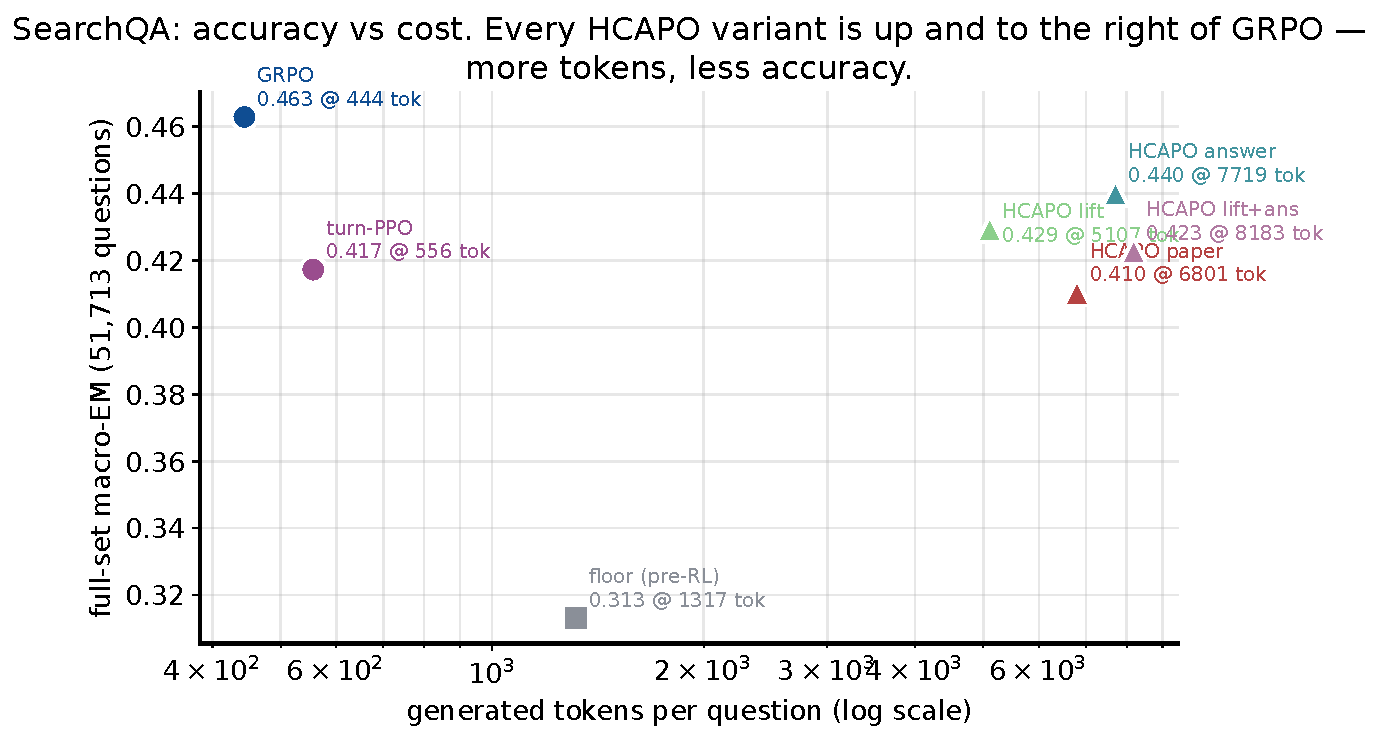
\includegraphics[width=0.82\linewidth]{figs/fig2_frontier.pdf}
\caption{Accuracy against token cost. Every HCAPO variant sits up and to the right of GRPO: more
tokens, less accuracy. The best HCAPO configuration spends $17\times$ GRPO's tokens to score
$0.023$ lower.}
\end{figure}

\noindent\textbf{ALFWorld} (Qwen3-1.7B, RL from a shared replay-BC policy, unseen 134 games):
turn-PPO $0.963$, GiGPO $0.955$, GRPO $0.881$, \textbf{HCAPO (paper-correct) $0.784$}, token-PPO
$0.761$. The corrected implementation did improve \emph{training}-set behaviour markedly over our
buggy one (seen-val peak $0.922$ vs $0.859$) --- but the advantage vanished on held-out games
($0.784$ vs $0.791$), i.e.\ it generalised no better. Its failure is concentrated on the
longest-horizon task type, \texttt{pick\_two\_obj\_and\_place}: $0.308$, against $1.000$ for both
GiGPO and turn-PPO --- precisely where per-turn credit should help most.

\begin{figure}[h]\centering\fig{fig5_hops.pdf}
\caption{Horizon-stratified SearchQA EM within the two multi-hop-spanning tasks. HCAPO tracks or
trails the baselines at every hop count; the deep-chain collapse (MuSiQue 4-hop) is not mitigated.}
\end{figure}

\section{Did the length-corrected variant help?}
Partly, and instructively. Against its own control (same $s_{final}$, only $m_t$ differs):

\begin{center}\small
\begin{tabular}{lccc}
\toprule
score on $s_{final}$=last\_obs & ignition step & final tokens & final clip\\
\midrule
hind (published) & 165 & 1742 & 0.75\\
\good{lift ($\Delta m$)} & \good{460} & \good{1420} & \good{0.65}\\
\bottomrule
\end{tabular}
\end{center}

\noindent It held $\sim$530--650 tokens for 300 consecutive steps --- six flat measurements --- and
posted the best mid-training accuracy of any HCAPO run ($0.447$ at step 350, level with GRPO's
endpoint). Then it ignited between steps 450 and 500. Full-set macro-EM $0.429$: better than the
published form's $0.410$, worse than the answer-injection form's $0.440$, and below GRPO's $0.463$.
The lift$\times$answer cell completed last: final val-EM $0.411$ at the cap (2047 tokens,
clip $\approx$1.0), full-set macro-EM $0.423$ --- slotting between the other HCAPO variants and
changing no conclusion. Final full-set ordering: GRPO $0.463>$ GiGPO $0.446>$ HCAPO
(hind,answer) $0.440>$ (lift,last\_obs) $0.429>$ (lift,answer) $0.423>$ turn-PPO $0.417>$
(hind,last\_obs) $0.410$.

The static diagnostic had predicted the lift would behave \emph{identically} to Eq.~6 (Spearman
$0.97$ co-ranking). It did not --- so rank-equivalence at a policy snapshot does not imply
equivalent training dynamics. That is a genuine, reusable finding about how to evaluate credit
estimators offline: snapshot rankings are insufficient; the feedback loop must be simulated.


\section{The full comparative suite}
This section reproduces, for the HCAPO arms, every analysis of the cross-environment report
(\texttt{2026-07-21\_4b\_horizon\_eval}): training curves, per-task accuracy, turn behaviour,
accuracy-vs-turns, spend-vs-need, and the stratified-horizon analyses with cluster-bootstrap
horizon-gain contrasts. All SearchQA arms here are protocol-matched (non-thinking@2048, 500 steps,
seed 0) with \textbf{GRPO as the $\Delta$-reference}; the thinking-protocol GiGPO/token-PPO rows of
\S4 are excluded from the matched contrasts.

\subsection{Training curves}
\begin{figure}[H]\centering\fig{fig_training_curves.pdf}
\caption{\emph{Left:} AlfWorld seen success — both HCAPO legs (orange/red) climb like the others
but plateau lower; the paper-correct leg peaks 0.922@145 vs the buggy 0.859. \emph{Right:} SearchQA
val-EM — every HCAPO arm tracks GRPO until its runaway ignites, then oscillates below it.}
\end{figure}

\subsection{Per-task accuracy}
\begin{table}[H]\centering\footnotesize\setlength{\tabcolsep}{4.2pt}
\caption{SearchQA full-set EM per task (51{,}713 q, non-thinking protocol). Best per column
\good{green}. GRPO leads every task except Bamboogle; the answer-injection arm is the closest HCAPO
on five of seven tasks.}
\begin{tabular}{lcccccccc}
\toprule
method & NQ & TriviaQA & PopQA & HotpotQA & 2Wiki & MuSiQue & Bamb. & \textbf{macro}\\
\midrule
pre-RL floor  & 0.292 & 0.517 & 0.346 & 0.271 & 0.331 & 0.074 & 0.360 & 0.313\\
\good{GRPO}   & \good{0.490} & \good{0.645} & \good{0.482} & \good{0.459} & \good{0.464} & \good{0.188} & 0.512 & \good{\textbf{0.463}}\\
turn-PPO      & 0.473 & 0.638 & 0.472 & 0.409 & 0.419 & 0.142 & 0.368 & 0.417\\
HCAPO hind+obs & 0.455 & 0.609 & 0.449 & 0.397 & 0.395 & 0.159 & 0.408 & 0.410\\
HCAPO hind+ans & 0.480 & 0.640 & 0.466 & 0.429 & 0.446 & 0.178 & 0.440 & 0.440\\
HCAPO lift+obs & 0.449 & 0.621 & 0.475 & 0.422 & 0.405 & 0.170 & 0.464 & 0.429\\
HCAPO lift+ans & 0.455 & 0.636 & 0.471 & 0.430 & 0.430 & 0.145 & 0.392 & 0.423\\
\bottomrule
\end{tabular}
\end{table}

\subsection{Turn behaviour}
\begin{figure}[H]\centering
\begin{minipage}{0.44\linewidth}\fig{fig2_alfworld_turns.pdf}\end{minipage}\hfill
\begin{minipage}{0.54\linewidth}\fig{fig3_searchqa_turns_box.pdf}\end{minipage}
\caption{\emph{Left:} AlfWorld trajectory length — both HCAPO legs sit at $\sim$17 turns, between
GRPO's wandering (14.9) and token-PPO's collapse (24.2), far above GiGPO/turn-PPO ($\sim$9--11).
\emph{Right:} SearchQA turns per dataset — the HCAPO arms saturate the 4-turn budget like GRPO,
but (unlike GRPO) largely via truncated non-action turns.}
\end{figure}

\noindent\textbf{AlfWorld by task type} (unseen success): the $\rho$ fix \emph{redistributed}
failure rather than removing it. The paper-correct leg recovered \texttt{examine}
($0.421\!\to\!0.789$) but collapsed \texttt{pick\_two} --- the longest-horizon type --- from the
buggy leg's $0.769$ to \textbf{0.308}, against $1.000$ for GRPO/GiGPO/turn-PPO. Net unseen change:
$0.791\to0.784$.

\subsection{Accuracy vs turns used}
\begin{figure}[H]\centering\fig{fig_acc_vs_turns_bothenv.pdf}
\caption{\emph{Left:} AlfWorld — every method solves $\approx$100\% of episodes finishing
$\le$20 turns; the ranking is set entirely by how often each drags past 20. Both HCAPO legs have
heavy $>$20 tails. \emph{Right:} SearchQA — the HCAPO arms cluster at 4 turns (cap saturation);
accuracy falls with turns used for all methods.}
\end{figure}

\subsection{Turns used vs required hops}
\begin{figure}[H]\centering\fig{fig4_searchqa_turns_vs_gold.pdf}
\caption{Turns used vs required hops (accurate / failed / all; band $\pm$1SD). The HCAPO arms pin
at the cap regardless of $H_{gold}$ --- they no longer \emph{modulate} search effort with question
depth, unlike GRPO/turn-PPO whose failed trajectories escalate with hops.}
\end{figure}

\subsection{Horizon-stratified accuracy and the horizon-gain contrasts}
\begin{figure}[H]\centering\fig{fig_a1_score_vs_hops.pdf}
\caption{EM vs required hops, pooled and within the two multi-hop-spanning tasks
(protocol-matched arms).}
\end{figure}

\begin{table}[H]\centering\small
\caption{Within-task EM by $H_{gold}$ (full-set). \good{Green} marks HCAPO cells that beat GRPO
\emph{absolutely}: the answer-injection arm wins every deep stratum.}
\begin{tabular}{lccc c cc}
\toprule
& \multicolumn{3}{c}{MuSiQue} && \multicolumn{2}{c}{2Wiki}\\
\cmidrule(lr){2-4}\cmidrule(lr){6-7}
& H2 & H3 & H4 && H2 & H4\\
\midrule
GRPO           & 0.283 & 0.101 & 0.059 && 0.454 & 0.502\\
turn-PPO       & 0.219 & 0.064 & 0.049 && 0.422 & 0.409\\
HCAPO hind+obs & 0.240 & 0.088 & 0.044 && 0.392 & 0.408\\
HCAPO hind+ans & 0.255 & \good{0.112} & \good{0.064} && 0.418 & \good{0.546}\\
HCAPO lift+obs & 0.258 & 0.084 & 0.057 && 0.422 & 0.345\\
HCAPO lift+ans & 0.239 & 0.051 & 0.032 && 0.410 & 0.498\\
\bottomrule
\end{tabular}
\end{table}

\begin{table}[H]\centering\small
\caption{Horizon-gain contrasts vs GRPO, $\Delta_m(\text{high})-\Delta_m(\text{low})$, 1000-resample
cluster bootstrap; $^\star$ = 95\% CI excludes 0. \textbf{HCAPO hind+answer is the first arm in the
entire campaign with significant POSITIVE horizon-gain on all three scopes.}}
\begin{tabular}{lccc}
\toprule
method & within-MuSiQue & within-2Wiki & pooled\\
\midrule
turn-PPO       & $+0.036^\star$ & $-0.061^\star$ & $-0.064^\star$\\
HCAPO hind+obs & $+0.029^\star$ & $-0.032^\star$ & $-0.036^\star$\\
\good{HCAPO hind+ans} & \good{$+0.037^\star$} & \good{$+0.079^\star$} & \good{$+0.044^\star$}\\
HCAPO lift+obs & $+0.013$ & $-0.124^\star$ & $-0.096^\star$\\
HCAPO lift+ans & $+0.002$ & $+0.040^\star$ & $-0.002$\\
\bottomrule
\end{tabular}
\end{table}

\noindent\textbf{The one genuinely positive HCAPO result.} The answer-injection arm loses to GRPO
overall ($0.440$ vs $0.463$) --- but the loss is entirely concentrated on \emph{shallow} questions.
On every deep stratum it beats GRPO absolutely (MuSiQue-3: $0.112$ vs $0.101$; MuSiQue-4: $0.064$
vs $0.059$; 2Wiki-4hop: $0.546$ vs $0.502$, the best value of any arm in the campaign), and its
horizon-gain contrast is significantly positive pooled and within both tasks. Read against \S2--3:
by the end of training this arm is a max-search policy (4 turns, $\approx$3 searches on
everything, most turns truncated) --- indiscriminate evidence-gathering that wastes budget on
single-hops but pays on deep chains. Whether that is \emph{hindsight credit} working or simply the
runaway manufacturing a search-everything policy cannot be separated with one seed; but it is the
only configuration in six that moved the deep-chain numbers past GRPO.

\subsection{Spend vs need, and where the budget dies}
\begin{figure}[H]\centering\fig{fig_a3_spend_vs_need.pdf}
\caption{Median turns and searches vs required hops. GRPO and the HCAPO arms sit at the cap for
every stratum; turn-PPO and the floor under-spend.}
\end{figure}

\begin{table}[H]\centering\small
\caption{Cap-exhausted failures (episode used all 4 turns and still failed), by stratum. For
max-turn policies (GRPO, HCAPO) this tracks $1-$EM; the informative rows are the floor and
turn-PPO, which fail \emph{without} exhausting the budget.}
\begin{tabular}{lcccc}
\toprule
method & H1 & H2 & H3 & H4\\
\midrule
floor & 0.030 & 0.087 & 0.225 & 0.180\\
turn-PPO & 0.059 & 0.192 & 0.458 & 0.480\\
GRPO & 0.453 & 0.555 & 0.899 & 0.555\\
HCAPO hind+ans & 0.356 & 0.527 & 0.868 & 0.467\\
HCAPO lift+obs & 0.288 & 0.362 & 0.679 & 0.556\\
\bottomrule
\end{tabular}
\end{table}

\subsection{Turn distributions and secondary splits}
\begin{figure}[H]\centering\fig{fig_a4_turn_violins.pdf}
\caption{Turn-count distributions per task. The HCAPO arms show the cap-pile signature on every
dataset --- including the single-hop tasks where a calibrated policy stops early.}
\end{figure}
\begin{figure}[H]\centering\fig{fig_a5_secondary.pdf}
\caption{Secondary splits: HotpotQA bridge vs comparison, PopQA head vs tail popularity. The HCAPO
arms preserve the baselines' pattern (comparison $\gg$ bridge; head $>$ tail) at a lower level ---
no HCAPO-specific redistribution.}
\end{figure}

\subsection{Per-method verdicts (suite view)}
\begin{itemize}\itemsep2pt
\item \textbf{HCAPO hind+obs (published form):} dominated --- below GRPO on every task, no positive
horizon signal beyond the MuSiQue critic-style contrast ($+0.029$), worst SearchQA macro of the
family, and the AlfWorld replication loses \texttt{pick\_two} almost entirely (0.308).
\item \textbf{HCAPO hind+ans:} the interesting one. Overall $-0.023$ vs GRPO, but absolutely ahead
on every deep stratum with the campaign's only fully-positive horizon-gain --- at $17\times$ GRPO's
token cost and 100\% truncation. If anything from HCAPO merits a follow-up seed, it is this cell.
\item \textbf{HCAPO lift+obs / lift+ans (our variant):} the best-behaved dynamics (latest
ignitions, lowest clip) and mid-family accuracy, but no horizon advantage --- the lift trades away
the deep-chain gains along with the runaway pressure.
\item \textbf{turn-PPO / GRPO baselines:} unchanged from the cross-environment report --- GRPO wins
the aggregate; turn-PPO keeps the only \emph{calibrated} spend profile (turns scale with hops,
budget not exhausted).
\end{itemize}

\section{Verdict and what would actually fix it}
HCAPO as published did not reproduce in our hands, on its own benchmark or ours, with an
implementation we verified line-by-line against Eq.~6--7 ($\rho$ centred on 1.0, two-sided, both
clip bounds engaging). Its per-turn signal is dominated by length, leakage and position artifacts,
and it carries a length ratchet that no parameter-level intervention removed.

Every intervention we tested changes the \emph{gain} of the length gradient. The untested class is
the one that changes its \emph{direction}: score turns on a \textbf{fixed window} (or another
length-invariant statistic) so that padding cannot move $m_t$ at all; and \textbf{exclude the final
turn} from hindsight credit, which our measurements show is the top-credit turn 73\% of the time
for reasons of entailment rather than pivotal-ness.

\section*{Fine print}
Single seed per configuration. SearchQA: Qwen3-4B, non-thinking, 4-turn cap, 2048-token responses,
500 steps, identical harness for every arm; the GiGPO and token-PPO rows use the thinking protocol
and are marked. ALFWorld: Qwen3-1.7B, transcript prompt, 512-token cap, 150 steps, evaluated at
best-seen checkpoint (the same rule for every arm). The ALFWorld number selects step 145 on a
128-game validation, which is itself noisy. The HCAPO paper's benchmarks use short action-style
turns under tight caps and a different base model; our results are a statement about these two task
settings, not a general refutation. Data, figures and the rerunnable analysis:
\texttt{assets/build\_figures.py}; the complete timestamped trail --- including five premature
stability calls I recorded and retracted --- is in
\texttt{docs/reports/2026-07-21\_4b\_horizon\_eval/results/hcapo\_wave3\_preregistration.md}.
Companion documents: \texttt{2026-07-29\_hcapo\_implementation\_note/} (the $\rho$ denominator bug),
\texttt{2026-07-30\_hcapo\_length\_runaway/} (the runaway in plain language), and
\texttt{2026-07-21\_4b\_horizon\_eval/} (the GRPO/GiGPO/PPO cross-environment study).
\end{document}
